\chapter{Dense-by-Sparse Algorithms}
\label{chapter:algs}

The main focus of this thesis is on improving the performance of small dense-by-sparse matrix multiplication algorithms. It is necessary to finesse around the bottlenecks that constrain the approaches described in the previous chapter. The extra information which makes this possible is the sparsity pattern known at compile time. Figure~\ref{fig:dxsp} shows the different algorithms under consideration and the relationship between them. The starting point is the outer-product formulation generated from \texttt{libxsmm}. This can be immediately adapted into SparseMicrokernel, 

\begin{figure}[H]
  \centering
  

\usetikzlibrary{shapes,arrows}
\usetikzlibrary{decorations.pathreplacing}


% Define block styles
\tikzstyle{decision} = [diamond, draw, fill=blue!20, 
    text width=4.5em, text badly centered, node distance=3cm, inner sep=0pt]

\tikzstyle{block} = [rectangle, draw, fill=gray!20, 
    text width=7em, text centered, minimum height=3em]

\tikzstyle{line} = [draw, -latex']

\tikzstyle{cloud} = [draw, ellipse,fill=red!20, node distance=3cm,
    minimum height=2em]

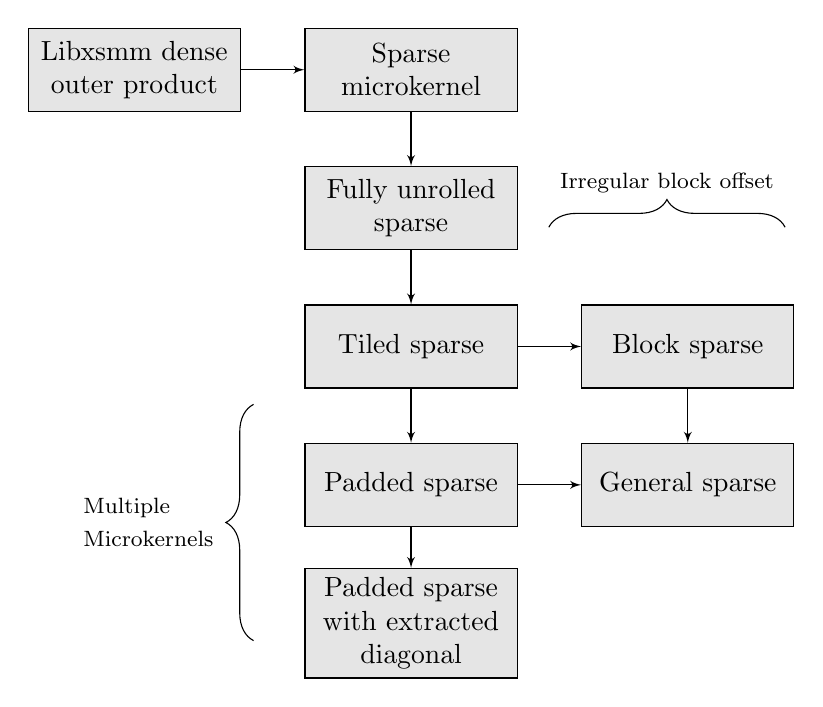
\begin{tikzpicture}[node distance = 5em, auto]
    % Place nodes

    \node [block] (microkernel) {Sparse\\ microkernel};
    \node [block, left of=microkernel, node distance=10em] (libxsmm) {Libxsmm dense outer product};
    \node [block, below of=microkernel] (macrokernel) {Fully unrolled\\ sparse};
    \node [block, below of=macrokernel] (tiledsparse) {Tiled sparse};
    \node [block, right of=tiledsparse, node distance=10em] (blocksparse) {Block sparse};
    \node [block, below of=tiledsparse] (paddedsparse) {Padded sparse};
    \node [block, below of=blocksparse] (generalsparse) {General sparse};
    \node [block, below of=paddedsparse] (paddeddiagsparse) {Padded sparse with extracted diagonal};

    %\node [block, left of=evaluate, node distance=3cm] (update) {update model};
    %\node [decision, below of=evaluate] (decide) {is best candidate better?};
    %\node [block, below of=decide, node distance=3cm] (stop) {stop};

    % Draw edges
    \path [line] (libxsmm) -- (microkernel);
    \path [line] (microkernel) -- (macrokernel);
    \path [line] (macrokernel) -- (tiledsparse);
    \path [line] (tiledsparse) -- (blocksparse);
    \path [line] (tiledsparse) -- (paddedsparse);
    \path [line] (paddedsparse) -- (generalsparse);
    \path [line] (blocksparse) -- (generalsparse);
    \path [line] (paddedsparse) -- (paddeddiagsparse);

    \draw [decorate,decoration={brace,amplitude=10pt},xshift=0pt,yshift=0pt]
(1.75,-2) -- (4.75,-2)node [black,midway,yshift=9pt] {\footnotesize Irregular block offset};

    \draw [decorate,decoration={brace,amplitude=10pt},xshift=0pt,yshift=0pt]
(-2,-7.25) -- (-2,-4.25) node [black,midway,xshift=-8pt,text width=5em] {\footnotesize Multiple\\ Microkernels};
    %\path [line] (evaluate) -- (decide);
    %\path [line] (decide) -| node [near start] {yes} (update);
    %\path [line] (update) |- (identify);
    %\path [line] (decide) -- node {no}(stop);
    %\path [line,dashed] (expert) -- (init);
    %\path [line,dashed] (system) -- (init);
    %\path [line,dashed] (system) |- (evaluate);
\end{tikzpicture}



  \label{fig:dxspfamilies}
  \caption{Relationships between different dense-by-sparse multiplication algorithms}
\end{figure}


\section{Sparse Microkernel}

The SparseMicrokernel is our first attempt to account for the sparsity pattern while building off of the state of the art for dense matrix multiplication. Our key assumption is that the matrices A and C are small enough to fit entirely in registers: $(n + k) * (m/8) <= 32$. Generating the dense GEMM for this problem effectively extracts the dense microkernel. This microkernel has no loops (otherwise it couldn't amortize the cost of loading and storing A and C) and this makes it easy to modify.

The sparse microkernel is a straightforward modification of the dense microkernel. All FMA instructions \texttt{C[:,ni] += A[:,ki] .* B[ki, ni]} where \texttt{B[ki, ni] = 0} due to the sparsity pattern are removed. This is tricky to do in a general way; an abstraction designed for the purpose is described at length in Section X.XX. Next, any loads of a column of A corresponding to an empty row of B are removed. Finally, any loads and stores of a column of C corresponding to an empty column of B are removed. This last step is often not desirable, as shall be discussed later, so the option is controlled by a parameter.

Now we consider the format of the sparse matrix B. Keeping B dense is suboptimal because the algorithm will be streaming adjacent nonzeros and it would be helpful if they occupied the same cache line. Breuer and Heinecke used a \emph{virtual} compressed sparse column format, where the nonzeros were laid out in a plain 1D array ordered by columns. For SparseMicrokernel, a virtual compressed row format might yield the best locality, but this is insignificant because few cache lines are involved on sparse matrices of this size. Having chosen the format, the next step is to choose an addressing scheme for the elements of the sparse matrix. The simplest scheme is to use pointer-offset addressing, where the pointer is in a register and the offset is hardcoded, such as \texttt{rsi + 22}. The downside of this approach is that when the offset is greater than 128*8, (i.e. there are more than 128 nonzeros in B), the resulting FMA instructions take up 10 bytes, which will cause a bottleneck as described in section X.XX. A more sophisticated scheme uses scale-index addressing, which uses two registers and two hardcoded values, such as \texttt{B + 8*i + 22}. These FMA instructions only take up 7 bytes; their main downside is that the generated code becomes harder to understand.

Another question is alignment. The alignment of B is not particularly important because its elements are loaded one at a time, but very important for A and C, which are loaded in a vectorwise fashion. If not aligned on a 64-byte boundary, the vector load operation will suffer a delay because the data is split across two cache lines. Using the aligned vector load operation \texttt{vmovapd} will trigger a segmentation fault if the pointer is not actually aligned. On the other hand, the unaligned version \texttt{vmovupd} can handle both the aligned and unaligned case, and will not incur the penalty if the pointer is in fact aligned. 

The performance of SparseMicrokernel shall be explored in Section X.XX. It is clear that removing the FMA instructions decreases the arithmetic intensity, and if the nonzeros are evenly distributed, there will be no accompanying decrease in memory bandwidth. Nevertheless the algorithm remains compute-bound and hence experiences an improved time-to-solution compared to its dense counterpart. Regardless of performance, SparseMicrokernel has limited utility in real problems, since it can only be applied to extremely small matrices. It is valuable primarily as a building block for the more complex algorithms developed next.

* What does the pseudocode look like?

\begin{itemize}
    \item Assume a dense A and a sparse B, with a fixed pattern known at compile time. As discussed in Section X.XX, 
    \item Pack B into a virtual compressed-sparse-row or column format
    \item Remove all fused-multiply-add and load instructions which are not needed
    \item Make this the basic building block for more complicated algorithms 
\end{itemize}




However, this has the following limitations:
\begin{itemize}
    \item Sparsity pattern must be known at compile time
    \item Pattern must fit within vector registers: $m \leq 8;  n \leq 30$
    \item (Dense $\times$ Sparse) $\neq$ (Sparse $\times$ Dense) due to vectorization
    \item Choice of row-major vs column-major format determines which of the two vectorizes nicely: $(AB)^T = B^T A^T$
\end{itemize}




The SparseMicrokernel algorithm is a straightforward modification: FMA instructions which operate on 
broadcasted zero entries are eliminated, and the memory addresses of the nonzero entries are 
shifted so that a sparse matrix format with better memory locality can be used. If an entire 
row of B is zero, the corresponding column of A is not needed, so the corresponding load 
operation is removed. Traversing the sparse matrix, finding the nonzeros, and finding the correct
memory address for each cell is done using a high-level cursor abstraction, as described elsewhere.   

Eliminating the unnecessary instructions reduces both computational intensity and memory traffic.


\begin{figure}[ht]
      \begin{minted}[fontsize=\footnotesize]{text}
        {text}
        loop over m blocks:

           unroll loop over n blocks:

              load C block into registers

              unroll loop over k blocks:

                 load A block into registers
                 microkernel for current B block
                 move A right 1 block
                 move B down 1 block

              store C block from registers
              move A to far left
              move B to top + right 1 block
              move C right 1 block

           move A down 1 block
           move C down 1 block
      \end{minted}
\end{figure}


\section{Unrolled dense-by-sparse multiplication}

Generate sparse microkernels for each (k,n) block of B, and unroll these into the instruction stream.
\begin{itemize}
      \item[$+$] Supports arbitrary matrix sizes
      \item[$+$] Dense-style register blocking for a dense $\times$ sparse algorithm.
      \item[$+$] Does not fill in any zeros -- no wasted flops

      \item[$-$] Generates an FMA instruction for each nonzero
      \item[$-$] These FMA instructions are 10B, too large to stream
      \item[$-$] Irregular location of blocks in memory prevents using tricks to reduce instruction size
      \item[$-$] Total number of nonzeros is limited by size of instruction cache.

\end{itemize}

\begin{figure}[tb]
  \centering
  \begin{subfigure}[b]{0.32\textwidth}
    \centering
          \[
      \left[
          \begin{array}{c c c | c c c }
          0 &   &   & 10 &   &   \\
          1 & 2 &   & 11& 12&   \\
            & 3 & 4 &   & 13& 14  \\
          \hline
          5 &   &   & 15  &   &   \\
          6 & 7 &   & 16  &17   &   \\
            & 8 & 9 &   & 18  &19   \\
          \end{array}
          \right]
      \]
    \caption{TiledSparse}
    \label{fig:tiledblocks}
  \end{subfigure}
  \begin{subfigure}[b]{0.32\textwidth}
    \centering
      \[
      \left[
          \begin{array}{c c c | c c c }
          0 &   &   &    &    &    \\
          1 & 2 &   &    &    &    \\
            & 3 & 4 &    &    &    \\
          \hline
          5 &   &   & 10 &    &    \\
          6 & 7 &   & 11 & 12 &    \\
            & 8 & 9 &    & 13 & 14 \\
          \end{array}
          \right]
      \]    \caption{BlockedSparse}
    \label{fig:blockedblocks}
  \end{subfigure}
    \begin{subfigure}[b]{0.32\textwidth}
    \centering
      \[
      \left[
          \begin{array}{c c c | c c c }
          0 &   &   &    &    &    \\
          1 & 2 &   &    &    &    \\
            & 3 & 4 &    &    &    \\
          \hline
          5  & 6  & 7  &    &  14& 15  \\
          8  & 9  & 10 &    &    & 16 \\
          11 & 12 & 13 &    &    &    \\
          \end{array}
          \right]
      \]    \caption{GeneralSparse}
    \label{fig:generalblocks}
  \end{subfigure}
  \caption{Sample matrices illustrating the blocking constraints for different GEMM algorithms. As shown in~\ref{fig:tiledblocks}, TiledSparse
  admits only a single block pattern which is tiled perfectly over the entire matrix. BlockedSparse admits a single block pattern along with empty blocks. GeneralSparse relaxes further to admit multiple different patterns. The numbers indicate the cell's index when using a block compressed-sparse-row format. }
  \label{fig:matrixblocks}

\end{figure}


\section{Tiled dense-by-sparse multiplication}

     The basic idea behind TiledSparse is to scale the FullyUnrolledSparse algorithm to 
matrices with more than 3100 nonzeros by assuming that the sparsity pattern is perfectly regular. 
Specifically, we assume that there is a single sparsity pattern which tiles over the entire matrix
and can be encoded as either a SparseMicrokernel or a FullyUnrolledSparse. The former, of course,
subjects the tiled sparsity pattern to register block size constraints, whereas the latter merely 
subjects it to number-of-nonzeros constraints. Our tiling assumption can be made without loss 
of generality because we can always fill in zeros until we arrive at a regular pattern. (One
way to do this is to partition the original matrix with a desired blocksize, and then take the 
logical union of the sparsity patterns in each block.) The assumption does result in a loss of 
practicality, however, as often the pattern will degenerate to dense. If the pattern is dense, 
and the pattern-blocksize is chosen sensibly, the resulting algorithm will be very similar to 
libxsmm.

There are several ways in which this algorithm may be modified. The first design variable is the
choice of loops to unroll. Because each pattern-block occupies the same amount of memory, the 
loops need only update the pointer to the current block, and thus may be unrolled trivially. 
The optimal amount of unrolling depends mainly on the number of nonzeros in the sparsity pattern.

The second design variable is the representation of the sparse matrix in memory. The choice will
directly affect both memory locality and FMA instruction size. (As discussed elsewhere, it is 
helpful to keep the pointer's offset under 128, as FMA instructions above that threshold are
10 bytes and below are 7 bytes.) A key constraint is regularity: This algorithm assumes it is
possible to traverse the matrix block-by-block using simple pointer arithmetic, which constrains 
the main layouts to (V){CSR, CSC, BCSR, BCSC}. (This assumption will be relaxed in 
later algorithms.) The layout which best suits the memory accesses made by TiledSparse 
is VBCSR. If the layout is prescribed externally as something other than (V){BCSR, BCSC), 
or if the pattern contains more than 128 nonzeros, it is recommended to use multiple cursors in 
order to keep the FMA instruction size down. One possible interoperability trick is to store 
the matrix in COO format, but order the values according to VBCSR. Of course, this is fragile 
if the matrix gets modified.

As mentioned earlier, the main limitation to this algorithm is the tendency for the block pattern to 
fill in until it becomes mostly dense. Otherwise, it is limited to having fewer than ~3000 nonzeros 
in the pattern. It does not require the tiling to be perfect (where the bottommost and rightmost 
tiles are full sized), although this makes the generator more complicated and reduces the allowed 
number of nonzeros in the pattern to $3000 - nnz(top_right) - nnz(bottom_right) - nnz(bottom_left)$. 



        Assume there exists a sparse pattern which tiles perfectly over B.
        \begin{itemize}
        \item[$+$] We can reuse a single microkernel, reducing the number of instructions
        \item[$+$] We can visit blocks in a loop efficiently, using pointer tricks to reduce instruction size.
        \item[$-$] This regularity assumption is likely too strong.
        \item[$-$] In practice, the sparsity pattern would often become dense.
        \end{itemize}




\section{Block dense-by-sparse multiplication}

  Assume that B is decomposed into blocks which are either empty or `full'. `Full' blocks all have the same sparsity pattern. This is a sparse generalization of the block-sparse-column format.

  \begin{itemize}
  \item[$+$] We can reuse a single microkernel, reducing the number of instructions
  \item[$+$] The zero blocks reduce the number of filled-in nonzeros.
  \item[$-$] We can no longer visit blocks by using a loop with pointer arithmetic. \\Our options are:
    \begin{itemize}
    \item Look up the block location from a table in memory
    \item Unroll the block locations into the instruction stream and repeatedly jump to the microkernel.
    \end{itemize}
  \end{itemize}




* What are the performance bottlenecks?
* What sparse matrix format constraints?
* What block size constraints?
* On which matrices is this likely to be efficient? On which matrices is this likely to be inefficient?


\section{General dense-by-sparse multiplication}

The general dense-by-sparse algorithm comes from relaxing \emph{both} of the TiledSparse constraints: There can be any number of different blocks, and each block may contain any number of nonzeros. GeneralSparse maintains a collection of SparseMicrokernel GEMMs 

This algorithm is subject to the following constraints:

\begin{enumerate}

  \item The total number of indirect jumps must be minimized. This implies that the total number of nonzero blocks should be as small as possible. 

  \item The routine must fit in the 32kB instruction cache, which constrains both the sum of nonzeros in each \emph{unique} block, as well as the total number of nonzero blocks. The latter constraint could possibly be finessed by storing the pointers to the start of each block and the corresponding GEMM routine in an array in the data cache instead of unrolling it into the instruction stream.

  \item The sparse matrix should be stored in \emph{block} compressed sparse row or column format in order to have good data locality.

  \item Blocks should be uniformly sized. This is an implementation detail; the constraint may be removed in the future by implementing another MatrixCursor as described in Section X.XX.

\end{enumerate}

Automatically choosing GeneralSparse parameters is ...

GeneralSparse degrades gracefully, similar to TiledSparse. As the matrices grow larger and denser, satisfying constraints (1) and (2) will lead to the unique blocks merging (and thereby filling in) until the algorithm resembles BlockSparse or TiledSparse. However, the overhead due to the indirect jumps means that BlockSparse or TiledSparse will prove to be more performant choice past a certain size.



\section{Extracted diagonal}

One pattern which emerges in sparse matrices is to 